\documentclass[aspectratio=169,11pt]{beamer}

% ================================================================
% "TABIIY TILNI QAYTA ISHLASH" KURSI
% MA'RUZA 3 --- Vektor fazo modellari, semantik munosabatlar va
%               ularni vizualizatsiya qilish
%              (d03_vektor_embedding.tex)
% Arxetiplar: [A][B][C][D][E] + 4 tsikl [F][G][H][I][J][K][L] +
%             [M][N][O][P][Q][R] + ilova [S]
% Rendered slayd soni: ~40 (4 kichik mavzuli rasmiy ma'ruza --- L1/L2 istisno precedentiga mos)
% Qulflangan [I2]: cos(a,b)=2/3~0.667 --- P3 (4-kun) birinchi assert manbayi.
%   Korpus: course_map.yaml hand_example verbatim:
%     a=(1,1,1,0) "nlp juda qiziq", b=(1,1,0,1) "nlp juda foydali",
%     V=(nlp, juda, qiziq, foydali)
% ================================================================

% ================================================================
% RANGLAR  (asl fayldan o'zgarishsiz)
% ================================================================
\definecolor{cnublue}{rgb}{0.07,0.14,0.62}
\definecolor{cnubluelight}{rgb}{0.18,0.30,0.72}
\definecolor{cnubluebg}{rgb}{0.90,0.92,0.97}
\definecolor{deepblue}{rgb}{0.07,0.14,0.62}
\definecolor{deepred}{rgb}{0.60,0.00,0.00}
\definecolor{deepgreen}{rgb}{0.00,0.45,0.00}
\definecolor{halfgray}{gray}{0.55}

% ================================================================
% BEAMER MAVZU --- Boadilla + maxsus footer  (asl fayldan o'zgarishsiz)
% ================================================================
\usetheme{Boadilla}

\setbeamercolor{structure}{fg=cnublue}
\setbeamercolor{frametitle}{bg=cnublue,fg=white}
\setbeamercolor{title}{bg=cnublue,fg=white}
\setbeamercolor{block title}{bg=cnublue,fg=white}
\setbeamercolor{block body}{bg=cnubluebg,fg=black}
\setbeamercolor{alerted text}{fg=deepred}
\setbeamercolor{author in head/foot}{bg=cnubluelight,fg=white}
\setbeamercolor{section in head/foot}{bg=cnublue,fg=white}
\setbeamercolor{page number in head/foot}{bg=cnubluelight,fg=white}

\setbeamertemplate{mini frame}{}
\setbeamertemplate{mini frame in current section}{}
\setbeamertemplate{mini frame in current subsection}{}
\setbeamertemplate{headline}{}
\setbeamertemplate{navigation symbols}{}

\setbeamertemplate{footline}{%
  \leavevmode%
  \hbox{%
    \begin{beamercolorbox}[wd=0.17\paperwidth,ht=2.5ex,dp=1.25ex,leftskip=0.5em]{author in head/foot}%
      \usebeamerfont{author in head/foot}\scriptsize\insertshortauthor%
    \end{beamercolorbox}%
    \begin{beamercolorbox}[wd=0.69\paperwidth,ht=2.5ex,dp=1.25ex,center]{section in head/foot}%
      \usebeamerfont{section in head/foot}%
      \scriptsize\insertsectionnavigationhorizontal{0.69\paperwidth}{}{}%
    \end{beamercolorbox}%
    \begin{beamercolorbox}[wd=0.14\paperwidth,ht=2.5ex,dp=1.25ex,rightskip=0.5em]{page number in head/foot}%
      \hfill\scriptsize\color{white}%
      \insertframenumber{}/\inserttotalframenumber%
    \end{beamercolorbox}%
  }%
  \vskip0pt%
}

% ================================================================
% PAKETLAR  (asl fayldan o'zgarishsiz)
% ================================================================
\usepackage[utf8]{inputenc}
\usepackage[T1]{fontenc}
\usepackage{lmodern}
\usepackage{amsmath,amssymb}
\usepackage{booktabs}
\usepackage{xcolor}
\usepackage{listings}
\lstset{
    language=Python,
    basicstyle=\ttfamily\scriptsize,
    keywordstyle=\bfseries\color{deepblue},
    emphstyle=\ttfamily\color{deepred},
    stringstyle=\color{deepgreen},
    commentstyle=\itshape\color{halfgray},
    numbers=left,
    numberstyle=\scriptsize\color{halfgray},
    rulesepcolor=\color{cnublue!30},
    frame=shadowbox,
    breaklines=true,
    showstringspaces=false,
    tabsize=2
}
\usepackage{tcolorbox}
\tcbuselibrary{skins}
\tcbset{
  defbox/.style={colback=cnubluebg,colframe=cnublue,
                 fonttitle=\small\bfseries\color{white},
                 attach boxed title to top left={yshift=-2mm,xshift=4mm},
                 boxed title style={colback=cnublue,colframe=cnublue}},
  warnbox/.style={colback=orange!8,colframe=orange!70!black,
                  fonttitle=\small\bfseries},
  okbox/.style={colback=green!7,colframe=green!55!black,
                fonttitle=\small\bfseries}
}
\usepackage{tikz}
\usetikzlibrary{arrows.meta,positioning}

% ================================================================
% QO'SHIMCHALAR  (asl fayldan o'zgarishsiz)
% ================================================================
\AtBeginSection[]{%
  \begin{frame}{Prezentatsiya rejasi}
    \tableofcontents[currentsection]
  \end{frame}}

\newcommand{\bunda}[1]{{\small\textbf{bunda:}\; #1}}
\newcommand{\bajarildi}{{\color{deepgreen}\large$\checkmark$}\;}

% ================================================================
% METAMA'LUMOT
% ================================================================
\title[Vektor fazo va embeddinglar]{Vektor fazo modellari va semantik munosabatlar}
\subtitle{Tabiiy tilni qayta ishlash --- 3-ma'ruza}
\author[A.A.\,Abdulali]{A.A.\,Abdulali}
\date{18-iyun 2026}
\institute{11:00--12:20 \quad$\cdot$\quad mavzu \textnumero{}3}

% ================================================================
\begin{document}
% ================================================================

% ----------------------------------------------------------------
% [A] TITUL
% ----------------------------------------------------------------
\maketitle

% ================================================================
\section[Kirish]{Kirish: TF-IDF dan embeddinggacha}
% ================================================================

% ----------------------------------------------------------------
% [B] TAKRORLASH: L2 va bugungi P2 dan ikki savol
% ----------------------------------------------------------------
\begin{frame}{Takrorlash: bugun ertalab nima qurdik?}
  \begin{columns}[T]
    \begin{column}{0.49\textwidth}
      \begin{tcolorbox}[warnbox,title=1-savol]
        \small
        P2 da sentiment klassifikatori \textbf{nima} ustida ishladi ---
        xom matn ustidami yoki vektor ustida?\\[3pt]
        \footnotesize Vektorni qaysi usul yaratdi?
      \end{tcolorbox}
    \end{column}
    \begin{column}{0.49\textwidth}
      \begin{tcolorbox}[warnbox,title=2-savol]
        \small
        TF-IDF fazosida \texttt{"qiziq"} va \texttt{"qiziqarli"}
        so'zlari bir-biriga \textbf{qanchalik yaqin}?
      \end{tcolorbox}
    \end{column}
  \end{columns}
  \pause
  \vspace{4pt}
  \begin{columns}[T]
    \begin{column}{0.49\textwidth}
      \begin{tcolorbox}[okbox,title=1-javob]
        \small
        Vektor ustida --- \textbf{TF-IDF / BoW} matritsasi.
        Model xom matnni emas, sonli vektorni ko'radi.
      \end{tcolorbox}
    \end{column}
    \begin{column}{0.49\textwidth}
      \begin{tcolorbox}[okbox,title=2-javob]
        \small
        \textbf{Umuman yaqin emas!} Ular ikki \textbf{alohida ustun} ---
        o'xshashligi $0$.\\
        \footnotesize\textcolor{halfgray}{TF-IDF so'z ma'nosini bilmaydi. Bugun shuni hal qilamiz.}
      \end{tcolorbox}
    \end{column}
  \end{columns}
\end{frame}

% ----------------------------------------------------------------
% [C] BUGUNGI MAQSADLAR
% ----------------------------------------------------------------
\begin{frame}{Siz bugungi dars oxirida quyidagilarni bajara olasiz:}
  \begin{enumerate}\setlength\itemsep{7pt}
    \item \textbf{Keltirib chiqara olasiz:} distributiv gipotezadan
          zich vektor (embedding) g'oyasini --- nega siyrak TF-IDF
          ma'noni ushlay olmaydi.
    \item \textbf{Qo'lda hisoblay olasiz:} ikki vektor orasidagi
          kosinus o'xshashlikni (kichik misol: $\cos = 2/3$).
    \item \textbf{Yecha olasiz:} vektor arifmetikasi bilan so'z
          analogiyasini ($\mathbf{b}-\mathbf{a}+\mathbf{c}$).
    \item \textbf{Kodda bog'lay olasiz:} \texttt{cosine\_similarity},
          \texttt{most\_similar} va \texttt{PCA} chaqiriqlarini
          formulaning qaysi qadami ekanligini ko'rsata olasiz.
  \end{enumerate}
  \vspace{4pt}
  \begin{tcolorbox}[defbox,title=Oldindan talab]
    \footnotesize
    L1 dan: BoW / TF-IDF vektori. Matematikadan: vektor, skalyar
    ko'paytma, norma (uzunlik). Eslamasangiz --- ilova slayd
    \textbf{S2} ga qarang.
  \end{tcolorbox}
\end{frame}

% ----------------------------------------------------------------
% [D] REJA VA VAQT BYUDJETI
% ----------------------------------------------------------------
\begin{frame}{Bugungi dars rejasi:}
  \begin{center}
  \small
  \begin{tabular}{c p{4.6cm} c p{3.4cm}}
    \toprule
    \textbf{Tsikl}& \textbf{Mavzu} & \textbf{Vaqt} & \textbf{Hosil bo'luvchi natija}\\
    \midrule
    1 & So'z embeddinglari: distributiv gipoteza, zich vektor & 18 daq & Embedding tushunchasi \\
    2 & Kosinus o'xshashligi & 22 daq & Qo'lda hisoblangan $\cos = 2/3$ \\
    3 & So'z analogiyalari va semantik munosabatlar & 18 daq & Vektor arifmetikasi \\
    4 & PCA bilan vizualizatsiya & 12 daq & 2D embedding fazosi \\
    \midrule
      & Xulosa va 3-amaliyotga ko'rsatmalar & 10 daq & Ertaga nima qurishingiz \\
    \bottomrule
  \end{tabular}
  \end{center}
  \vspace{4pt}
  \begin{tcolorbox}[warnbox,title=Har bir tsikl qanday qurilgan]
    \footnotesize\sloppy
    intuitsiya $\to$ rasmiy ta'rif $\to$ qo'lda misol $\to$ sizning
    vazifangiz $\to$ kod bilan ishlash uchun ko'prik. Bugungi
    $\cos = 2/3$ ertangi amaliyotda \texttt{assert} sifatida tekshiriladi.
  \end{tcolorbox}
\end{frame}

% ----------------------------------------------------------------
% [E] MUAMMO BIRINCHI: TF-IDF MA'NONI USHLAMAYDI
% ----------------------------------------------------------------
\begin{frame}{Bugungi dars uchun muammo: TF-IDF ``qiziq'' va ``qiziqarli'' ni butunlay begona deb biladi}
  \begin{columns}[T]
    \begin{column}{0.50\textwidth}
      \textbf{L1 oxirida savol qoldirgandik:}\\[4pt]
      \small\textit{``TF-IDF \texttt{qiziq} va \texttt{qiziqarli} ni
      bir xil ma'no deb ko'ra oladimi?''}\\[6pt]
      \begin{tcolorbox}[warnbox,title=Javob: yo'q!,top=2pt,bottom=2pt]
        \small
        Lug'atda ular ikki \textbf{alohida o'lcham}:\\[3pt]
        \texttt{qiziq}\;\;\;\,$\to (1, 0)$\\
        \texttt{qiziqarli} $\to (0, 1)$\\[3pt]
        Skalyar ko'paytma $= 0 \Rightarrow$ o'xshashlik $= 0$,
        ma'nosi yaqin bo'lsa ham.
      \end{tcolorbox}
    \end{column}
    \begin{column}{0.46\textwidth}
      \textbf{Yana ikki kamchilik:}\\[4pt]
      \small
      \begin{itemize}\setlength\itemsep{3pt}
        \item \textbf{Siyraklik}: vektor o'lchami $=|V|$ ---
              minglab nol.
        \item \textbf{Sinonim ko'rmaydi}: \texttt{avtomobil}
              $\ne$ \texttt{mashina}.
      \end{itemize}
      \vspace{5pt}
      \begin{tcolorbox}[okbox,title=Bugungi yechim,top=2pt,bottom=2pt]
        \footnotesize
        \textbf{Zich vektor (embedding)}: kichik o'lchamli, ma'noni
        ushlaydigan ifoda. O'xshash so'zlar --- yaqin vektorlar.
      \end{tcolorbox}
    \end{column}
  \end{columns}
\end{frame}

% ================================================================
\section[Embeddinglar]{Zich vektorlar: so'z embeddinglari}
% ================================================================

% ----------------------------------------------------------------
% [F1] INTUITSIYA: SIYRAK VS ZICH
% ----------------------------------------------------------------
\begin{frame}{So'zni qanday qilib raqamga aylantiramiz? Siyrakdan zichgacha}
  \begin{columns}[T]
    \begin{column}{0.50\textwidth}
      \textbf{Siyrak (one-hot / TF-IDF):}\\[4pt]
      \small
      \texttt{nlp} $\to (0,\ldots,1,\ldots,0)$\\[2pt]
      \footnotesize
      $|V|$ o'lchamli --- masalan 50\,000.\\
      Faqat bitta $1$, qolgani nol.\\
      Har so'z boshqalardan \textbf{teng uzoqlikda}.\\[6pt]
      \normalsize\textbf{Zich (embedding):}\\[4pt]
      \small
      \texttt{nlp} $\to (0.21,\,-0.08,\,0.66,\ldots)$\\[2pt]
      \footnotesize
      Kichik o'lchamli --- masalan 100--300.\\
      Barcha qiymatlar to'la (nol emas).\\
      O'xshash so'zlar --- \textbf{yaqin} vektorlar.
    \end{column}
    \begin{column}{0.46\textwidth}
      \begin{tcolorbox}[defbox,title=Distributiv gipoteza,top=2pt,bottom=2pt]
        \footnotesize
        \textit{``So'zni uning hamrohlaridan bilib olasan.''}\\
        (Firth, 1957)\\[4pt]
        O'xshash \textbf{kontekstda} uchraydigan so'zlar ---
        o'xshash ma'noga ega.
      \end{tcolorbox}
      \vspace{4pt}
      \footnotesize
      \texttt{choy}, \texttt{kofe} ko'pincha bir xil so'zlar bilan
      keladi: \textit{``issiq ___ ichdim''} $\Rightarrow$ vektorlari
      yaqin bo'lishi kerak.
    \end{column}
  \end{columns}
\end{frame}

% ----------------------------------------------------------------
% [G1] RASMIY TA'RIF: EMBEDDING
% ----------------------------------------------------------------
\begin{frame}{So'z embeddingi: rasmiy ta'rif}
  \begin{tcolorbox}[defbox,title=Ta'rif: so'z embeddingi (word embedding)]
    \textbf{Embedding} --- lug'atdagi har bir so'zni $d$ o'lchamli
    zich haqiqiy vektorga akslantiruvchi funksiya:
    $$ E : V \longrightarrow \mathbb{R}^{d}, \qquad d \ll |V| $$
    O'xshash ma'noli so'zlar fazoda \textbf{yaqin} joylashadi.
  \end{tcolorbox}
  \vspace{5pt}
  \bunda{%
    $V$ = lug'at; $|V|$ = lug'at hajmi (masalan 50\,000);
    $d$ = embedding o'lchami (masalan 100--300);
    $E(w)\in\mathbb{R}^d$ = $w$ so'zining vektori
  }
  \vspace{5pt}
  \begin{itemize}\small\setlength\itemsep{3pt}
    \item One-hot: $d = |V|$, faqat bitta $1$ --- ma'no \alert{yo'q}.
    \item Embedding: $d$ kichik, zich --- ma'no vektor \textbf{yo'nalishida}.
    \item Vektorlar matndan \textbf{o'rganiladi} (Word2Vec, GloVe --- L6, GloVe maqolasi).
  \end{itemize}
\end{frame}

% ----------------------------------------------------------------
% [H1] KELTIRIB CHIQARISH: NEGA ONE-HOT NING O'XSHASHLIGI HAR DOIM 0
% ----------------------------------------------------------------
\begin{frame}{Nega one-hot vektorlar ma'noni ushlay olmaydi?}
  \textbf{1-qadam.} Ikki har xil so'zning one-hot vektorlari:
  $$ \texttt{qiziq} \to \mathbf{u}=(1,0,0,\ldots), \qquad
     \texttt{qiziqarli} \to \mathbf{v}=(0,1,0,\ldots) $$
  \pause
  \textbf{2-qadam.} Skalyar ko'paytmasini hisoblaymiz:
  $$ \mathbf{u}\cdot\mathbf{v} = 1{\cdot}0 + 0{\cdot}1 + \cdots = 0
     \qquad\text{\scriptsize\color{halfgray}(umumiy ``faol'' o'lcham yo'q)} $$
  \pause
  \textbf{3-qadam.} Demak \textbf{istalgan} ikki har xil so'z uchun
  o'xshashlik $= 0$ --- ma'no qanchalik yaqin bo'lishidan qat'i nazar.
  \begin{tcolorbox}[okbox]
    \small \textbf{Xulosa:} one-hot fazosida ``yaqinlik'' tushunchasi
    yo'q. Embedding aynan shu bo'shliqni to'ldiradi --- vektorlarni
    ma'noga qarab \textbf{bir-biriga yaqinlashtiradi}. Endi
    ``yaqinlik''ni qanday \textbf{o'lchashni} ko'ramiz (2-tsikl).
  \end{tcolorbox}
\end{frame}

% ----------------------------------------------------------------
% [I1] QO'LDA MISOL: ONE-HOT vs ZICH
% ----------------------------------------------------------------
\begin{frame}{Qo'lda misol: bir xil so'zlar, ikki xil ifoda}
  \begin{columns}[T]
    \begin{column}{0.50\textwidth}
      \textbf{One-hot (siyrak):}\\[4pt]
      \small
      \texttt{qiziq}\;\;\;\,$\to \mathbf{u}=(1,0)$\\
      \texttt{qiziqarli} $\to \mathbf{v}=(0,1)$\\[5pt]
      $\mathbf{u}\cdot\mathbf{v} = 1{\cdot}0 + 0{\cdot}1 = \mathbf{0}$\\[3pt]
      \footnotesize Vektorlar \textbf{perpendikular} ---
      umuman bog'lanmagan.
    \end{column}
    \begin{column}{0.46\textwidth}
      \textbf{Zich (o'rgangan embedding):}\\[4pt]
      \small
      \texttt{qiziq}\;\;\;\,$\to \mathbf{a}=(0.9,\,0.4)$\\
      \texttt{qiziqarli} $\to \mathbf{b}=(0.8,\,0.5)$\\[5pt]
      $\mathbf{a}\cdot\mathbf{b} = 0.72 + 0.20 = \mathbf{0.92}$\\[3pt]
      \footnotesize Vektorlar \textbf{deyarli bir yo'nalishda} ---
      ma'nosi yaqin.
    \end{column}
  \end{columns}
  \vspace{6pt}
  \begin{tcolorbox}[okbox,title=Muhim kuzatuv,top=2pt,bottom=2pt]
    \footnotesize
    Bir xil ikki so'z: one-hot da o'xshashlik $0$, zich embeddingda
    yuqori. Yo'nalishni \textbf{sonli} o'lchash uchun --- keyingi
    tsiklda kosinus o'xshashligi.
  \end{tcolorbox}
\end{frame}

% ----------------------------------------------------------------
% [J1] SIZNING VAZIFANGIZ: DISTRIBUTIV MULOHAZA
% ----------------------------------------------------------------
\begin{frame}{Sizning vazifangiz: qaysi juft yaqinroq?}
  \begin{tcolorbox}[warnbox,title=Savol --- 60 soniya]
    \small
    Distributiv gipotezaga ko'ra, embedding fazosida qaysi juft so'z
    bir-biriga \textbf{yaqinroq} bo'lishi kerak?\\[5pt]
    (a) \texttt{(avtomobil, mashina)} \qquad
    (b) \texttt{(avtomobil, banan)}\\[4pt]
    \footnotesize Qarorni qanday asoslaysiz?
  \end{tcolorbox}
  \pause
  \begin{tcolorbox}[okbox,title=Javob]
    \small
    \textbf{(a) \texttt{(avtomobil, mashina)}.}\\[3pt]
    Bu ikki so'z bir xil kontekstlarda uchraydi:
    \textit{``yangi ___ sotib oldim''}, \textit{``___ ni haydadi''}.
    Kontekstlari o'xshash $\Rightarrow$ vektorlari yaqin.\\[3pt]
    \texttt{banan} esa butunlay boshqa kontekstda
    (\textit{``meva''}, \textit{``yedim''}) $\Rightarrow$ uzoq vektor.
  \end{tcolorbox}
\end{frame}

% ================================================================
\section[Kosinus]{Kosinus o'xshashligi}
% ================================================================

% ----------------------------------------------------------------
% [F2] INTUITSIYA: BURCHAK
% ----------------------------------------------------------------
\begin{frame}{Intuitsiya: o'xshashlik --- bu vektorlar orasidagi burchak}
  \begin{columns}[T]
    \begin{column}{0.52\textwidth}
      \begin{center}
      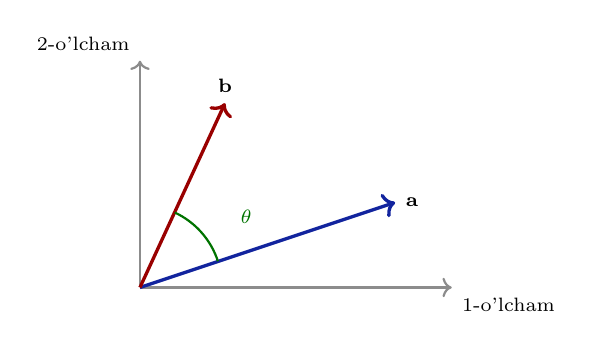
\begin{tikzpicture}[scale=0.9]
        \draw[->,thick,draw=halfgray] (0,0)--(4.4,0)
              node[below right]{\scriptsize 1-o'lcham};
        \draw[->,thick,draw=halfgray] (0,0)--(0,3.2)
              node[above left]{\scriptsize 2-o'lcham};
        \draw[->,very thick,draw=cnublue]  (0,0)--(3.6,1.2)
              node[right]{\scriptsize $\mathbf{a}$};
        \draw[->,very thick,draw=deepred] (0,0)--(1.2,2.6)
              node[above]{\scriptsize $\mathbf{b}$};
        \draw[draw=deepgreen,thick] (1.1,0.37) arc (18:65:1.15);
        \node[color=deepgreen] at (1.5,1.0) {\scriptsize $\theta$};
      \end{tikzpicture}
      \end{center}
    \end{column}
    \begin{column}{0.44\textwidth}
      \textbf{Asosiy g'oya (so'z bilan):}
      \begin{itemize}\setlength\itemsep{4pt}
        \item Har so'z (yoki hujjat) --- fazodagi \textbf{vektor}
        \item O'xshashlik = vektorlar orasidagi \textbf{burchak}
        \item Burchak kichik $\Rightarrow$ ma'no yaqin
        \item Burchak $90^\circ$ $\Rightarrow$ bog'lanmagan
      \end{itemize}
      \vspace{0.2em}
      \begin{tcolorbox}[okbox,top=2pt,bottom=2pt]
        \small \textbf{Nega burchak, uzunlik emas?} Uzun hujjat ham,
        qisqasi ham bir mavzuda bo'lishi mumkin --- burchak buni
        adolatli o'lchaydi.
      \end{tcolorbox}
    \end{column}
  \end{columns}
\end{frame}

% ----------------------------------------------------------------
% [G2] RASMIY TA'RIF: KOSINUS + BUNDA
% ----------------------------------------------------------------
\begin{frame}{Kosinus o'xshashligi: rasmiy ta'rif}
  \begin{tcolorbox}[defbox,title=Ta'rif: kosinus o'xshashligi (cosine similarity)]
    \vspace{-0.6em}
    $$\cos(\mathbf{a},\mathbf{b})
      = \frac{\mathbf{a}\cdot\mathbf{b}}
             {\lVert\mathbf{a}\rVert\,\lVert\mathbf{b}\rVert}
      = \frac{\sum_{i=1}^{n} a_i b_i}
             {\sqrt{\sum_{i=1}^{n} a_i^2}\,\sqrt{\sum_{i=1}^{n} b_i^2}}$$
  \end{tcolorbox}
  \vspace{0.2em}
  \bunda{$\mathbf{a},\mathbf{b}\in\mathbb{R}^n$ --- vektorlar
  (TF-IDF yoki embedding); $n$ --- o'lcham; $\mathbf{a}\cdot\mathbf{b}$
  --- skalyar ko'paytma; $\lVert\cdot\rVert$ --- Evklid normasi (uzunlik).}
  \vspace{0.5em}
  \begin{itemize}\small\setlength\itemsep{3pt}
    \item Qiymatlar oralig'i: $[-1,\,1]$; TF-IDF manfiy emas
          $\Rightarrow$ amalda $[0,\,1]$.
    \item $\cos = 1$: bir xil yo'nalish; $\cos = 0$: umumiy o'lcham yo'q.
  \end{itemize}
\end{frame}

% ----------------------------------------------------------------
% [H2] KELTIRIB CHIQARISH: NEGA AYNAN SHU FORMULA
% ----------------------------------------------------------------
\begin{frame}{Keltirib chiqarish: nega normaga bo'lamiz?}
  \textbf{1-qadam.} Skalyar ko'paytmaning geometrik ta'rifi:
  $$\mathbf{a}\cdot\mathbf{b}
    = \lVert\mathbf{a}\rVert\,\lVert\mathbf{b}\rVert\cos\theta
    \qquad\text{\scriptsize\color{halfgray}(chiziqli algebradan)}$$
  \pause
  \textbf{2-qadam.} Bizga kerak bo'lgan $\cos\theta$ ni ajratamiz:
  $$\cos\theta
    = \frac{\mathbf{a}\cdot\mathbf{b}}
           {\lVert\mathbf{a}\rVert\,\lVert\mathbf{b}\rVert}
    \qquad\text{\scriptsize\color{halfgray}(ikkala tomonni normalarga bo'ldik)}$$
  \pause
  \textbf{3-qadam.} Vektorni ikki marta uzaytirsak ($\mathbf{a}'=2\mathbf{a}$):
  $$\cos(\mathbf{a}',\mathbf{b})
    = \frac{2(\mathbf{a}\cdot\mathbf{b})}
           {2\lVert\mathbf{a}\rVert\,\lVert\mathbf{b}\rVert}
    = \cos(\mathbf{a},\mathbf{b})$$
  \begin{tcolorbox}[okbox]
    \small \textbf{Xulosa:} kosinus uzunlikka \textbf{bog'liq emas} ---
    faqat yo'nalishni o'lchaydi. Aynan shuning uchun matn va NLP da
    standart o'xshashlik o'lchovi.
  \end{tcolorbox}
\end{frame}

% ----------------------------------------------------------------
% [I2] QO'LDA HISOB --- QULFLANGAN TRACEABILITY SLAYD
%
% P3 (kun-4) birinchi assert bilan solishtiring:
%   cos(a,b) = 2/3 ~ 0.667   [Ma'ruza L3 [I2]-slayd]
% Korpus: course_map.yaml hand_example verbatim:
%   a=(1,1,1,0) "nlp juda qiziq", b=(1,1,0,1) "nlp juda foydali"
%   V = (nlp, juda, qiziq, foydali)
% ----------------------------------------------------------------
\begin{frame}{Qo'lda hisob: ikki vektorning kosinus o'xshashligi}
  \begin{tcolorbox}[defbox,title=Kichik korpus (BoW vektorlari)]
    \small
    $H_1$: \texttt{"nlp juda qiziq"} $\;\to\; \mathbf{a}=(1,1,1,0)$\quad
    $H_2$: \texttt{"nlp juda foydali"} $\;\to\; \mathbf{b}=(1,1,0,1)$\\[2pt]
    {\scriptsize\color{halfgray}Lug'at tartibi:
    (\texttt{nlp}, \texttt{juda}, \texttt{qiziq}, \texttt{foydali})}
  \end{tcolorbox}
  \vspace{0.2em}
  \begin{columns}[T]
    \begin{column}{0.50\textwidth}
      \textbf{Hisoblaymiz:}
      \begin{align*}
        \mathbf{a}\cdot\mathbf{b} &= 1{\cdot}1 + 1{\cdot}1 + 1{\cdot}0 + 0{\cdot}1 = 2\\
        \lVert\mathbf{a}\rVert &= \sqrt{1+1+1+0} = \sqrt{3}\\
        \lVert\mathbf{b}\rVert &= \sqrt{1+1+0+1} = \sqrt{3}
      \end{align*}
    \end{column}
    \begin{column}{0.46\textwidth}
      \textbf{Natija:}
      $$\cos = \frac{2}{\sqrt{3}\sqrt{3}} = \frac{2}{3} \approx \mathbf{0.667}$$
      \begin{tcolorbox}[okbox,top=2pt,bottom=2pt]
        \footnotesize 4 so'zdan 2 tasi (\texttt{nlp}, \texttt{juda})
        mos --- intuitsiya bilan ham $\approx 2/3$ chiqishi tabiiy.
      \end{tcolorbox}
      \vspace{3pt}
      \footnotesize\color{halfgray}
      Ertangi P3 birinchi assert:\\
      \texttt{abs(cos\_val - 0.667) < 1e-3}\\
      \textit{\# Ma'ruza L3 [I2]-slayd}
    \end{column}
  \end{columns}
\end{frame}

% ----------------------------------------------------------------
% [J2] SIZNING VAZIFANGIZ: KOSINUS
% ----------------------------------------------------------------
\begin{frame}{Sizning vazifangiz: kosinusni hisoblang}
  \begin{tcolorbox}[warnbox,title=Savol --- 2 daqiqa]
    \small
    $H_1$: \texttt{"nlp juda qiziq"}
    $\;\to\;\mathbf{a}=(1,1,1,0,0,0)$\\[3pt]
    $H_3$: \texttt{"python juda qulay"}
    $\;\to\;\mathbf{c}=(0,1,0,0,1,1)$\\[3pt]
    {\scriptsize\color{halfgray}Lug'at: (\texttt{nlp}, \texttt{juda},
    \texttt{qiziq}, \texttt{foydali}, \texttt{python}, \texttt{qulay})}\\[5pt]
    \textbf{\large $\cos(\mathbf{a},\mathbf{c})$ ni hisoblang.}
  \end{tcolorbox}
  \pause
  \begin{tcolorbox}[okbox,title=Javob]
    \small
    $\mathbf{a}\cdot\mathbf{c} = 1$ (faqat \texttt{juda} mos);\quad
    $\lVert\mathbf{a}\rVert = \lVert\mathbf{c}\rVert = \sqrt{3}$\\[3pt]
    $\cos = \dfrac{1}{\sqrt{3}\sqrt{3}} = \dfrac{1}{3} \approx \mathbf{0.333}$\\[3pt]
    $H_1$ va $H_3$ faqat ``juda'' da mos --- mavzu boshqa
    (\texttt{nlp} vs \texttt{python}) $\Rightarrow$ past o'xshashlik.
  \end{tcolorbox}
\end{frame}

% ----------------------------------------------------------------
% [K2] KOD <-> FORMULA: cosine_similarity  [fragile]
% ----------------------------------------------------------------
\begin{frame}[fragile]{Kod $\leftrightarrow$ formula: har qator formulaning qaysi qismi?}
  \begin{columns}[T]
    \begin{column}{0.52\textwidth}
      \begin{lstlisting}
import numpy as np
from sklearn.metrics.pairwise \
    import cosine_similarity

a = np.array([[1, 1, 1, 0]])
b = np.array([[1, 1, 0, 1]])

# (1) skalyar ko'paytma
skalyar = (a * b).sum()      # 2
# (2) normalar
na = np.linalg.norm(a)       # 1.732
nb = np.linalg.norm(b)       # 1.732
# (3) kosinus = (1) / (2)
print(skalyar / (na * nb))   # 0.667

# bitta qatorda:
print(cosine_similarity(a, b))
      \end{lstlisting}
    \end{column}
    \begin{column}{0.44\textwidth}
      \textbf{Moslik jadvali:}
      \vspace{0.2em}
      \begin{center}\scriptsize
      \begin{tabular}{ll}
        \toprule
        \textbf{Kod} & \textbf{Formula} \\
        \midrule
        \texttt{(a*b).sum()} & $\sum_i a_i b_i$ \\
        \texttt{norm(a)} & $\lVert\mathbf{a}\rVert$ \\
        \texttt{skalyar/(na*nb)} & $\cos(\mathbf{a},\mathbf{b})$ \\
        \bottomrule
      \end{tabular}
      \end{center}
      \vspace{0.3em}
      \begin{tcolorbox}[okbox,top=2pt,bottom=2pt]
        \small Ertangi P3 da xuddi shu hisob \textbf{haqiqiy
        embedding vektorlarda} bajariladi --- bugungi $2/3$ uning
        birlik testi (sanity check) bo'ladi.
      \end{tcolorbox}
    \end{column}
  \end{columns}
\end{frame}

% ----------------------------------------------------------------
% [L2] TUZOG': 1D massiv shakli  [fragile]
% ----------------------------------------------------------------
\begin{frame}[fragile]{Kosinus tuzog'i: 1D massiv \texttt{cosine\_similarity} ni sindiradi}
  \begin{columns}[T]
    \begin{column}{0.50\textwidth}
      \begin{tcolorbox}[warnbox,title=Haqiqiy xato --- tez-tez uchraydi]
        \small
        \texttt{cosine\_similarity} \textbf{2D} massiv kutadi
        (\textit{(namuna, o'lcham)} shaklida). 1D bersak --- xato.
      \end{tcolorbox}
      \vspace{3pt}
      \footnotesize\color{halfgray}
      Embedding vektori odatda 1D (\texttt{shape=(100,)}) bo'lib
      keladi --- shuning uchun bu xato amaliyotda ko'p uchraydi.
    \end{column}
    \begin{column}{0.46\textwidth}
      \begin{lstlisting}[numbers=none,frame=single,
                         basicstyle=\ttfamily\scriptsize]
a = np.array([1, 1, 1, 0])
cosine_similarity(a, b)
# XATO: Expected 2D array!

# To'g'ri: (1, n) shaklga keltiring
cosine_similarity(
    a.reshape(1, -1),
    b.reshape(1, -1))
      \end{lstlisting}
    \end{column}
  \end{columns}
\end{frame}

% ================================================================
\section[Analogiyalar]{So'z analogiyalari va semantik munosabatlar}
% ================================================================

% ----------------------------------------------------------------
% [F3] INTUITSIYA: VEKTOR ARIFMETIKASI
% ----------------------------------------------------------------
\begin{frame}{Intuitsiya: ma'no farqi --- vektorlar orasidagi yo'nalish}
  \begin{columns}[T]
    \begin{column}{0.52\textwidth}
      \begin{center}
      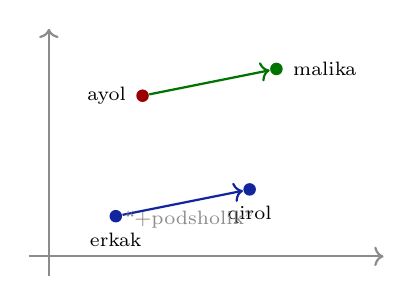
\begin{tikzpicture}[scale=0.85]
        \draw[->,thick,draw=halfgray] (-0.3,0)--(5,0);
        \draw[->,thick,draw=halfgray] (0,-0.3)--(0,3.4);
        \node[circle,fill=cnublue,inner sep=1.6pt,label=below:{\scriptsize erkak}] (m) at (1,0.6) {};
        \node[circle,fill=cnublue,inner sep=1.6pt,label=below:{\scriptsize qirol}] (k) at (3,1) {};
        \node[circle,fill=deepred,inner sep=1.6pt,label=left:{\scriptsize ayol}] (w) at (1.4,2.4) {};
        \node[circle,fill=deepgreen,inner sep=1.6pt,label=right:{\scriptsize malika}] (q) at (3.4,2.8) {};
        \draw[->,thick,cnublue] (m)--(k);
        \draw[->,thick,deepgreen] (w)--(q);
        \node[font=\scriptsize,color=halfgray] at (2.1,0.55) {``+podsholik''};
      \end{tikzpicture}
      \end{center}
    \end{column}
    \begin{column}{0.44\textwidth}
      \textbf{Asosiy g'oya:}\\[3pt]
      \small
      Bir xil \textbf{munosabat} --- bir xil \textbf{yo'nalish} vektori.\\[5pt]
      \texttt{qirol} $-$ \texttt{erkak} $\approx$
      \texttt{malika} $-$ \texttt{ayol}\\[5pt]
      Mashhur misol (ingliz):\\
      \footnotesize
      \texttt{king} $-$ \texttt{man} $+$ \texttt{woman}
      $\approx$ \texttt{queen}.\\[4pt]
      \normalsize Embedding fazosi semantik munosabatlarni
      \textbf{geometrik} saqlaydi.
    \end{column}
  \end{columns}
\end{frame}

% ----------------------------------------------------------------
% [G3] RASMIY TA'RIF: ANALOGIYA + BUNDA
% ----------------------------------------------------------------
\begin{frame}{So'z analogiyasi: rasmiy ta'rif}
  \begin{tcolorbox}[defbox,title=Ta'rif: analogiya (``a : b :: c : ?'')]
    ``$a$ ga $b$ qanday bo'lsa, $c$ ga \textbf{nima} shunday'' savoliga
    javob vektor:
    $$ \mathbf{t} = \mathbf{b} - \mathbf{a} + \mathbf{c}, \qquad
       \hat{d} = \arg\max_{w \in V \setminus \{a,b,c\}}
                 \cos\!\big(E(w),\, \mathbf{t}\big) $$
  \end{tcolorbox}
  \vspace{4pt}
  \bunda{$\mathbf{a}=E(a)$, $\mathbf{b}=E(b)$, $\mathbf{c}=E(c)$ ---
  so'z vektorlari; $\mathbf{t}$ --- maqsad vektor;
  $\hat{d}$ --- $\mathbf{t}$ ga kosinus bo'yicha eng yaqin so'z.}
  \vspace{5pt}
  \begin{itemize}\small\setlength\itemsep{3pt}
    \item $\mathbf{b}-\mathbf{a}$ --- ``$a$ dan $b$ ga'' munosabat yo'nalishi.
    \item Uni $\mathbf{c}$ ga qo'shamiz $\Rightarrow$ kerakli mintaqaga boramiz.
    \item Eng yaqin so'zni \textbf{kosinus} bilan topamiz (2-tsikl ishlaydi!).
  \end{itemize}
\end{frame}

% ----------------------------------------------------------------
% [H3] KELTIRIB CHIQARISH: ANALOGIYA QADAMMA-QADAM
% ----------------------------------------------------------------
\begin{frame}{Analogiyani qadamma-qadam yechamiz}
  \textbf{Savol:} \texttt{uzbekiston : toshkent :: rossiya : ?}
  (poytaxt munosabati)
  \vspace{4pt}
  \textbf{1-qadam.} Munosabat yo'nalishini topamiz:
  $$ \mathbf{b} - \mathbf{a} = E(\texttt{toshkent}) - E(\texttt{uzbekiston})
     \quad\text{\scriptsize\color{halfgray}(``davlat $\to$ poytaxt'' yo'nalishi)} $$
  \pause
  \textbf{2-qadam.} Uni yangi davlatga qo'llaymiz:
  $$ \mathbf{t} = \mathbf{b} - \mathbf{a} + \mathbf{c}
     = E(\texttt{toshkent}) - E(\texttt{uzbekiston}) + E(\texttt{rossiya}) $$
  \pause
  \textbf{3-qadam.} $\mathbf{t}$ ga eng yaqin so'zni qidiramiz:
  $$ \hat{d} = \arg\max_{w} \cos(E(w), \mathbf{t}) \;=\; \texttt{moskva} $$
  \begin{tcolorbox}[okbox,top=2pt,bottom=2pt]
    \small Embedding ``poytaxt'' munosabatini hech kim aytmasdan,
    faqat matndan o'rgangan --- bu distributiv gipotezaning kuchli isboti.
  \end{tcolorbox}
\end{frame}

% ----------------------------------------------------------------
% [I3] QO'LDA HISOB: ANALOGIYA (2D)
% ----------------------------------------------------------------
\begin{frame}{Qo'lda hisob: analogiyani 2D vektorlarda yechamiz}
  \begin{tcolorbox}[defbox,title=Kichik embedding fazosi (2D)]
    \small
    $E(\texttt{uzbekiston})=(2,0)$,\quad $E(\texttt{toshkent})=(3,1)$,\quad
    $E(\texttt{rossiya})=(6,0)$\\[2pt]
    Nomzodlar: $E(\texttt{moskva})=(7,1)$,\quad $E(\texttt{parij})=(9,5)$
  \end{tcolorbox}
  \vspace{0.2em}
  \begin{columns}[T]
    \begin{column}{0.52\textwidth}
      \textbf{Maqsad vektor:}
      \begin{align*}
        \mathbf{t} &= \mathbf{b}-\mathbf{a}+\mathbf{c}\\
          &= (3,1)-(2,0)+(6,0)\\
          &= (7,\,1)
      \end{align*}
    \end{column}
    \begin{column}{0.46\textwidth}
      \textbf{Eng yaqinini topamiz:}\\[3pt]
      \small
      $\mathbf{t}=(7,1)$ ga:\\
      \texttt{moskva}$=(7,1)$ --- aynan mos!\\
      \texttt{parij}$=(9,5)$ --- uzoq.\\[4pt]
      $\Rightarrow \hat{d}=\texttt{moskva}$
    \end{column}
  \end{columns}
  \vspace{4pt}
  \begin{tcolorbox}[okbox,title=Javob,top=2pt,bottom=2pt]
    \footnotesize
    \texttt{uzbekiston : toshkent :: rossiya : \textbf{moskva}} ---
    poytaxt munosabati vektor arifmetikasi bilan topildi.
  \end{tcolorbox}
\end{frame}

% ----------------------------------------------------------------
% [J3] SIZNING VAZIFANGIZ: ANALOGIYA
% ----------------------------------------------------------------
\begin{frame}{Sizning vazifangiz: analogiyani yeching}
  \begin{tcolorbox}[warnbox,title=Savol --- 2 daqiqa]
    \small
    $E(\texttt{erkak})=(1,1)$,\quad $E(\texttt{qirol})=(3,2)$,\quad
    $E(\texttt{ayol})=(1,3)$\\[3pt]
    Nomzodlar: $E(\texttt{malika})=(3,4)$,\quad $E(\texttt{dehqon})=(2,1)$\\[5pt]
    \textbf{\large \texttt{erkak : qirol :: ayol : ?}}
  \end{tcolorbox}
  \pause
  \begin{tcolorbox}[okbox,title=Javob]
    \small
    $\mathbf{t}=\mathbf{b}-\mathbf{a}+\mathbf{c}
      = (3,2)-(1,1)+(1,3) = (3,\,4)$\\[3pt]
    $\mathbf{t}=(3,4)$ ga eng yaqin: \texttt{malika}$=(3,4)$ (aynan mos)
    $\gg$ \texttt{dehqon}$=(2,1)$.\\[3pt]
    $\Rightarrow$ \texttt{erkak : qirol :: ayol : \textbf{malika}}.
  \end{tcolorbox}
\end{frame}

% ----------------------------------------------------------------
% [K3] KOD <-> FORMULA: gensim most_similar  [fragile]
% ----------------------------------------------------------------
\begin{frame}[fragile]{Kod $\leftrightarrow$ formula: \texttt{most\_similar} va analogiya}
  \begin{columns}[T]
    \begin{column}{0.54\textwidth}
\begin{lstlisting}
from gensim.models import KeyedVectors

wv = KeyedVectors.load("cc_uz_100k.kv")

# Eng o'xshash so'zlar (kosinus bilan)
wv.most_similar("toshkent", topn=3)

# Analogiya: b - a + c
# uzbekiston:toshkent :: rossiya:?
wv.most_similar(
    positive=["toshkent", "rossiya"],
    negative=["uzbekiston"],
    topn=1)
# -> [("moskva", 0.78)]
\end{lstlisting}
    \end{column}
    \begin{column}{0.42\textwidth}
      \textbf{Argument $\to$ formula:}\\[4pt]
      \footnotesize
      \begin{tabular}{p{2.3cm}l}
        \toprule
        Kod & Formula \\
        \midrule
        \texttt{positive=[c, b]} & $+\mathbf{c}+\mathbf{b}$ \\
        \texttt{negative=[a]} & $-\mathbf{a}$ \\
        \texttt{most\_similar} & $\arg\max \cos$ \\
        \bottomrule
      \end{tabular}
      \vspace{4pt}
      \begin{tcolorbox}[warnbox,title=Eslatma,top=2pt,bottom=2pt]
        \footnotesize
        \texttt{positive} $=$ qo'shiladigan,
        \texttt{negative} $=$ ayriladigan vektorlar.
        P3 da aynan shu API ishlatiladi.
      \end{tcolorbox}
    \end{column}
  \end{columns}
\end{frame}

% ================================================================
\section[Vizualizatsiya]{PCA bilan vizualizatsiya}
% ================================================================

% ----------------------------------------------------------------
% [F4] INTUITSIYA: 300D NI KO'RA OLMAYMIZ
% ----------------------------------------------------------------
\begin{frame}{Intuitsiya: 300 o'lchamli fazoni qanday ``ko'ramiz''?}
  \begin{columns}[T]
    \begin{column}{0.50\textwidth}
      \textbf{Muammo:}\\[3pt]
      \small
      Embedding $100$--$300$ o'lchamli.\\
      Inson faqat $2$--$3$ o'lchamni ko'radi.\\[6pt]
      \textbf{Yechim --- PCA:}\\[3pt]
      Yuqori o'lchamli nuqtalarni eng ko'p \textbf{tarqalish}
      (varianta) saqlanadigan $2$ o'lchamga \textbf{proyeksiya} qiladi.
    \end{column}
    \begin{column}{0.46\textwidth}
      \begin{center}
      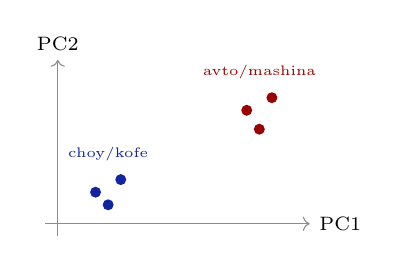
\begin{tikzpicture}[scale=0.8]
        \draw[->,draw=halfgray] (-0.2,0)--(4,0) node[right]{\scriptsize PC1};
        \draw[->,draw=halfgray] (0,-0.2)--(0,2.6) node[above]{\scriptsize PC2};
        \node[circle,fill=cnublue,inner sep=1.4pt] at (0.6,0.5) {};
        \node[circle,fill=cnublue,inner sep=1.4pt] at (1.0,0.7) {};
        \node[circle,fill=cnublue,inner sep=1.4pt] at (0.8,0.3) {};
        \node[font=\tiny,cnublue] at (0.8,1.1) {choy/kofe};
        \node[circle,fill=deepred,inner sep=1.4pt] at (3.0,1.8) {};
        \node[circle,fill=deepred,inner sep=1.4pt] at (3.4,2.0) {};
        \node[circle,fill=deepred,inner sep=1.4pt] at (3.2,1.5) {};
        \node[font=\tiny,deepred] at (3.2,2.4) {avto/mashina};
      \end{tikzpicture}
      \end{center}
      \footnotesize\color{halfgray}
      Semantik klasterlar 2D da ko'rinadi --- o'xshash so'zlar guruhlanadi.
    \end{column}
  \end{columns}
\end{frame}

% ----------------------------------------------------------------
% [G4] RASMIY TA'RIF: PCA (NAZARIY) + BUNDA
% ----------------------------------------------------------------
\begin{frame}{PCA: asosiy komponentlar tahlili (nazariy ta'rif)}
  \begin{tcolorbox}[defbox,title=Ta'rif: PCA (Principal Component Analysis)]
    \small
    PCA --- ma'lumotni \textbf{eng katta varianta} yo'nalishlari bo'ylab
    yangi o'qlarga (asosiy komponentlarga) burib, faqat birinchi $k$
    o'qni saqlaydigan o'lcham qisqartirish usuli.
  \end{tcolorbox}
  \vspace{4pt}
  \bunda{markazlashtirilgan ma'lumot $X$; kovariatsiya matritsasi
  $C=\frac{1}{n}X^\top X$; asosiy komponentlar --- $C$ ning eng katta
  xos qiymatlariga mos xos vektorlari; $k$ --- saqlanadigan o'lcham (bizda $2$).}
  \vspace{5pt}
  \begin{itemize}\small\setlength\itemsep{3pt}
    \item PC1 --- varianta eng katta bo'lgan yo'nalish.
    \item PC2 --- PC1 ga perpendikular, qolgan eng katta varianta.
    \item \texttt{explained\_variance\_ratio\_} --- har komponent
          qancha ``ma'lumot'' saqlaganini ko'rsatadi.
  \end{itemize}
\end{frame}

% ----------------------------------------------------------------
% [I4] QO'LDA MISOL: PCA INTUITSIYASI
% ----------------------------------------------------------------
\begin{frame}{Qo'lda misol: qaysi o'q ko'proq ma'lumot saqlaydi?}
  \begin{tcolorbox}[defbox,title=Uchta nuqta (2D, markazlashtirilgan)]
    \small
    $w_1=(2,\;0.1)$,\qquad $w_2=(-2,\;-0.1)$,\qquad $w_3=(0,\;0)$
  \end{tcolorbox}
  \vspace{0.2em}
  \begin{columns}[T]
    \begin{column}{0.52\textwidth}
      \textbf{Har o'q bo'ylab tarqalish:}
      \begin{align*}
        \mathrm{Var}(x) &\propto 2^2 + (-2)^2 + 0^2 = 8\\
        \mathrm{Var}(y) &\propto 0.1^2 + 0.1^2 + 0^2 = 0.02
      \end{align*}
      \footnotesize $x$ o'qida tarqalish $\approx 400$ marta katta.
    \end{column}
    \begin{column}{0.46\textwidth}
      \textbf{Xulosa:}\\[3pt]
      \small
      PC1 $\approx x$ o'qi (deyarli barcha varianta).\\[3pt]
      2D $\to$ 1D: faqat $x$ ni saqlaymiz:\\
      $w_1\to 2$,\; $w_2\to -2$,\; $w_3\to 0$.\\[3pt]
      Nuqtalar farqi \textbf{saqlanib qoldi}, $y$ deyarli yo'qotilmadi.
    \end{column}
  \end{columns}
  \vspace{3pt}
  \begin{tcolorbox}[okbox,top=2pt,bottom=2pt]
    \footnotesize
    PCA aynan shuni avtomatik qiladi: kam ma'lumotli o'qni tashlab,
    ko'p ma'lumotli o'qni saqlaydi. Bu yerda \texttt{explained\_variance}
    $\approx 8/8.02 \approx 99.8\%$.
  \end{tcolorbox}
\end{frame}

% ----------------------------------------------------------------
% [J4] SIZNING VAZIFANGIZ: PCA NIMANI YO'QOTADI
% ----------------------------------------------------------------
\begin{frame}{Sizning vazifangiz: PCA nimani saqlaydi, nimani yo'qotadi?}
  \begin{tcolorbox}[warnbox,title=Savol --- 90 soniya]
    \small
    $300$ o'lchamli o'zbek embeddinglari PCA bilan $2$ o'lchamga
    tushirildi va \texttt{explained\_variance\_ratio\_} $=[0.31,\,0.18]$
    chiqdi.\\[5pt]
    (a) Vizualizatsiya ma'lumotning qancha qismini saqladi?\\
    (b) Ikki so'z 2D rasmda yaqin ko'rinsa, ular embedding fazosida
        ham yaqinligi \textbf{kafolatlanadimi}?
  \end{tcolorbox}
  \pause
  \begin{tcolorbox}[okbox,title=Javob]
    \small
    (a) Atigi $0.31 + 0.18 = \mathbf{0.49}$ --- ya'ni $\approx 49\%$.
    Qolgan $51\%$ tarqalish (nozik farqlar) \textbf{yo'qoladi}.\\[3pt]
    (b) \textbf{Yo'q.} 2D yaqinlik --- taxminiy. To'liq fazoda uzoq
    so'zlar proyeksiyada tasodifan yaqin tushishi mumkin. Aniq
    qaror uchun \textbf{to'liq vektorda} kosinusni hisoblang.
  \end{tcolorbox}
\end{frame}

% ----------------------------------------------------------------
% [K4] KOD <-> FORMULA: PCA + scatter  [fragile]
% ----------------------------------------------------------------
\begin{frame}[fragile]{Kod $\leftrightarrow$ formula: PCA bilan 2D vizualizatsiya}
  \begin{columns}[T]
    \begin{column}{0.56\textwidth}
\begin{lstlisting}
from sklearn.decomposition import PCA
import matplotlib.pyplot as plt

# X: (so'zlar_soni, 100) embedding matritsa
pca = PCA(n_components=2)   # k = 2
xy = pca.fit_transform(X)   # -> (N, 2)

plt.scatter(xy[:, 0], xy[:, 1])
for i, soz in enumerate(sozlar):
    plt.annotate(soz, xy[i])

print(pca.explained_variance_ratio_)
# -> [0.41, 0.22]  (jami ~63%)
\end{lstlisting}
    \end{column}
    \begin{column}{0.40\textwidth}
      \textbf{Kod $\to$ tushuncha:}\\[3pt]
      \footnotesize
      \begin{tabular}{p{2.0cm}p{2.0cm}}
        \toprule
        Kod & Ma'no \\
        \midrule
        \texttt{n\_components=2} & $k=2$ o'q \\
        \texttt{fit\_transform} & proyeksiya \\
        \texttt{variance\_ratio\_} & saqlangan ulush \\
        \bottomrule
      \end{tabular}
      \vspace{4pt}
      \begin{tcolorbox}[warnbox,title=Eslatma,top=2pt,bottom=2pt]
        \footnotesize
        2 komponent ko'pincha ma'lumotning
        atigi yarmini saqlaydi --- vizualizatsiya
        \textbf{taxminiy}, isbot emas.
      \end{tcolorbox}
    \end{column}
  \end{columns}
\end{frame}

% ================================================================
\section[Xulosa]{Xulosa va amaliyotga ko'prik}
% ================================================================

% ----------------------------------------------------------------
% [M] O'ZBEK TILIGA XOSLIK (majburiy arxetip)
% ----------------------------------------------------------------
\begin{frame}{Tayyor embeddinglar o'zbek tili uchun cheklangan qamrovga ega}
  \begin{columns}[T]
    \begin{column}{0.50\textwidth}
      \textbf{Asosiy muammo:}\\[4pt]
      \small
      Mashhur GloVe / Word2Vec vektorlari asosan \textbf{ingliz}
      korpusida o'qitilgan.\\[4pt]
      O'zbek so'zlarining ko'pi ularda \alert{umuman yo'q} (OOV ---
      out of vocabulary).\\[4pt]
      Agglutinatsiya buni kuchaytiradi:\\
      \texttt{kitob}, \texttt{kitoblar}, \texttt{kitobimizdan} ---
      \textbf{har biri} alohida (yoki yo'q) vektor.
    \end{column}
    \begin{column}{0.46\textwidth}
      \begin{tcolorbox}[warnbox,title=OOV ta'siri,top=2pt,bottom=2pt]
        \footnotesize
        OOV so'z $\to$ vektor yo'q $\to$ o'xshashlik hisoblanmaydi.
        Ertaga P3 da \texttt{oov\_rate()} ni o'lchaysiz --- o'zbek
        korpusida u yuqori chiqadi.
      \end{tcolorbox}
      \vspace{4pt}
      \textbf{Yechimlar:}\\[3pt]
      \footnotesize
      \begin{itemize}\setlength\itemsep{2pt}
        \item O'zbek korpusida \textbf{noldan} o'qitish (L6, P6).
        \item Stemming bilan shakllarni birlashtirish (m01).
        \item Subword (FastText / BPE) --- OOV ni kamaytiradi (4-hafta).
      \end{itemize}
    \end{column}
  \end{columns}
\end{frame}

% ----------------------------------------------------------------
% [N] SINTEZ: SIYRAK vs ZICH TAQQOSLOV
% ----------------------------------------------------------------
\begin{frame}{Qachon nima ishlatamiz? Siyrak va zich vektorlar taqqoslovi}
  \begin{center}\small
  \begin{tabular}{p{3.0cm}p{4.2cm}p{4.2cm}}
    \toprule
    \textbf{Mezon} & \textbf{Siyrak (TF-IDF / BoW)} & \textbf{Zich (embedding)} \\
    \midrule
    O'lcham & $|V|$ (katta) & $d=100$--$300$ (kichik) \\
    Ma'no & Ushlamaydi & Ushlaydi (yaqinlik) \\
    Sinonim & Begona ($\cos=0$) & Yaqin vektor \\
    OOV (yangi so'z) & 0-ustun (xavfsiz) & Vektor yo'q (muammo) \\
    Talqin qilish & Oson (so'z = o'lcham) & Qiyin (yashirin o'lcham) \\
    O'zbek uchun & Stemming kerak & Korpus + qamrov muhim \\
    Qachon & Klassik ML, kichik data & Semantik qidiruv, neyron model \\
    \bottomrule
  \end{tabular}
  \end{center}
  \vspace{4pt}
  \begin{tcolorbox}[okbox,title=Amaliy qoida,top=2pt,bottom=2pt]
    \footnotesize
    Kichik, oddiy vazifa $\Rightarrow$ TF-IDF bilan boshlang.
    Ma'no, o'xshashlik, semantik qidiruv kerak bo'lsa $\Rightarrow$
    embedding. Ikkalasida ham kosinus o'xshashlik o'lchovi ishlaydi.
  \end{tcolorbox}
\end{frame}

% ----------------------------------------------------------------
% [O] SEMINAL MAQOLA + MUHOKAMA SAVOLI
% ----------------------------------------------------------------
\begin{frame}{Seminal maqola: GloVe (Pennington va b., 2014)}
  \begin{tcolorbox}[defbox,title=Seminal maqola]
    \small
    Pennington, J., Socher, R., Manning, C.D.\ (2014).
    \textbf{GloVe: Global Vectors for Word Representation.}
    \textit{EMNLP 2014}.
  \end{tcolorbox}
  \vspace{5pt}
  \textbf{Maqola haqida:}
  \begin{itemize}\small\setlength\itemsep{3pt}
    \item So'zlarning \textbf{global} birga-uchrash (co-occurrence)
          statistikasidan zich vektor o'rganadi.
    \item Word2Vec lokal oynadan, GloVe esa butun matritsadan o'rganadi.
    \item Analogiya vazifalarida (\texttt{king$-$man$+$woman}) kuchli natija.
    \item Bugungi BERT, GPT ham ``embedding'' g'oyasiga tayanadi.
  \end{itemize}
  \vspace{5pt}
  \begin{tcolorbox}[warnbox,title=Muhokama savoli (P3 gacha o'ylang)]
    \small
    Ingliz korpusida o'qitilgan GloVe o'zbek so'zlari uchun deyarli
    foydasiz. Kam-resursli o'zbek tili uchun \textbf{qaysi} afzal:
    tayyor inglizcha vektorni moslashtirishmi yoki o'zbek korpusida
    noldan o'qitishmi? Nega?
  \end{tcolorbox}
\end{frame}

% ----------------------------------------------------------------
% [P] MAQSADLAR BAJARILDI
% ----------------------------------------------------------------
\begin{frame}{Bugungi maqsadlar bajarildi}
  \begin{enumerate}\setlength\itemsep{9pt}
    \item \bajarildi \textbf{Keltirib chiqardik:}
          distributiv gipotezadan zich vektor (embedding) g'oyasini ---
          one-hot o'xshashligi nega har doim $0$.
    \item \bajarildi \textbf{Hisobladik:}
          ikki vektorning kosinus o'xshashligi ---
          $\cos(\mathbf{a},\mathbf{b}) = 2/3 \approx 0.667$ ([I2]-slayd).
    \item \bajarildi \textbf{Yechdik:}
          vektor arifmetikasi bilan analogiya ---
          \texttt{uzbekiston:toshkent :: rossiya:moskva}.
    \item \bajarildi \textbf{Kodda bog'ladik:}
          \texttt{cosine\_similarity}, \texttt{most\_similar} va
          \texttt{PCA} chaqiriqlarini formulaga moslashtirdik.
  \end{enumerate}
\end{frame}

% ----------------------------------------------------------------
% [Q] KO'PRIK: ERTAGA P3
% ----------------------------------------------------------------
\begin{frame}{Ertaga P3: tayyor embeddinglar bilan ishlaysiz}
  \begin{center}
  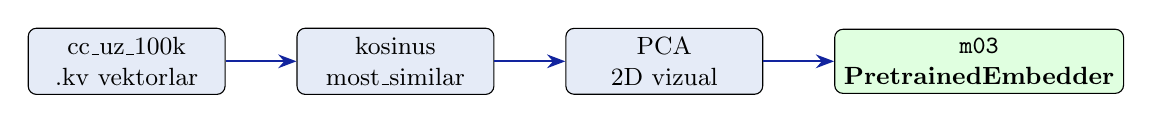
\begin{tikzpicture}[
      mod/.style={draw, fill=cnubluebg, rounded corners=3pt,
                  minimum width=2.5cm, minimum height=0.75cm,
                  font=\small, align=center},
      fin/.style={draw, fill=green!12, rounded corners=3pt,
                  minimum width=2.5cm, minimum height=0.75cm,
                  font=\small\bfseries, align=center},
      arr/.style={-{Stealth}, thick, color=cnublue}
  ]
    \node[mod] (kv)  {cc\_uz\_100k\\.kv vektorlar};
    \node[mod, right=0.9cm of kv]  (sim) {kosinus\\most\_similar};
    \node[mod, right=0.9cm of sim] (pca) {PCA\\2D vizual};
    \node[fin, right=0.9cm of pca] (cap) {\texttt{m03}\\PretrainedEmbedder};
    \draw[arr] (kv)--(sim);
    \draw[arr] (sim)--(pca);
    \draw[arr] (pca)--(cap);
  \end{tikzpicture}
  \end{center}
  \vspace{6pt}
  \begin{columns}[T]
    \begin{column}{0.50\textwidth}
      \textbf{P3 da qurasiz:}\\[3pt]
      \small
      \begin{itemize}\setlength\itemsep{2pt}
        \item \texttt{KeyedVectors} bilan \texttt{.kv} yuklash
        \item \texttt{most\_similar}, analogiya yechish
        \item \texttt{oov\_rate()} --- o'zbek qamrovi
        \item PCA bilan semantik klasterlarni chizish
        \item \texttt{m03\_pretrained\_embedder.py} saqlash
      \end{itemize}
    \end{column}
    \begin{column}{0.46\textwidth}
      \textbf{Birinchi assert (bu slayd [I2]):}\\[4pt]
      \small\ttfamily
      assert abs(cos\_val - 0.667) < 1e-3\\[4pt]
      \normalfont\footnotesize\color{halfgray}
      \textit{\# Ma'ruza L3 [I2]-slayd bilan}\\
      \textit{\# solishtiring}\\[5pt]
      \normalfont\footnotesize Tayyorlab keling: Kaggle hisobi ishlashini
      tekshiring; muhokama savoliga [O] javob.
    \end{column}
  \end{columns}
\end{frame}

% ----------------------------------------------------------------
% [R] ADABIYOTLAR
% ----------------------------------------------------------------
\begin{frame}{Adabiyotlar}
  \begin{enumerate}\small\setlength\itemsep{6pt}
    \item Pennington, J., Socher, R., Manning, C.D.\ (2014).
          \textit{GloVe: Global Vectors for Word Representation.}
          EMNLP 2014.
    \item Mikolov, T. va b.\ (2013).
          \textit{Efficient Estimation of Word Representations in
          Vector Space.} ICLR 2013. (Word2Vec --- L6 da batafsil.)
    \item Jurafsky, D., Martin, J.H.\ (2023).
          \textit{Speech and Language Processing}, 3-nashr (online).
          6-bob: Vector Semantics and Embeddings.
    \item Firth, J.R.\ (1957). \textit{A Synopsis of Linguistic Theory.}
          (Distributiv gipoteza manbasi.)
    \item Scikit-learn hujjatlari: \texttt{cosine\_similarity},
          \texttt{PCA} --- scikit-learn.org.
  \end{enumerate}
\end{frame}

% ================================================================
% [S] ILOVALAR (appendix --- slayd soniga kirmaydi)
% ================================================================
\appendix

\begin{frame}{Ilova S1: kosinus va Evklid masofa bog'liqligi}
  \small
  $L_2$-normallashtirilgan vektorlar uchun
  ($\lVert\mathbf{a}\rVert=\lVert\mathbf{b}\rVert=1$):
  $$\lVert\mathbf{a}-\mathbf{b}\rVert^2
    = \lVert\mathbf{a}\rVert^2 + \lVert\mathbf{b}\rVert^2
      - 2\,\mathbf{a}\cdot\mathbf{b}
    = 2 - 2\cos(\mathbf{a},\mathbf{b})$$
  \bunda{$\lVert\mathbf{a}\rVert=\lVert\mathbf{b}\rVert=1$ deb olindi.}
  \vspace{4pt}

  Demak normallashtirilgan fazoda Evklid masofasi va kosinus
  \textbf{ekvivalent tartib} beradi --- shuning uchun ko'p kutubxonalar
  ikkalasini almashtirib ishlatadi. Bu LSH va qidiruvda muhim (L4, P4).
\end{frame}

\begin{frame}{Ilova S2: vektor, norma va skalyar ko'paytma eslatmasi}
  \begin{tcolorbox}[defbox,title=Kerakli tushunchalar]
    \small
    Skalyar ko'paytma: $\mathbf{a}\cdot\mathbf{b}=\sum_i a_i b_i$\\[3pt]
    Evklid normasi (uzunlik): $\lVert\mathbf{a}\rVert=\sqrt{\sum_i a_i^2}$\\[3pt]
    Perpendikular vektorlar: $\mathbf{a}\cdot\mathbf{b}=0$
  \end{tcolorbox}
  \vspace{4pt}
  \small\textbf{Misol:} $\mathbf{a}=(3,4)$ uchun
  $\lVert\mathbf{a}\rVert=\sqrt{9+16}=\sqrt{25}=5$.\\[3pt]
  Python da: \texttt{import numpy as np; np.linalg.norm([3,4])} $\to 5.0$;\quad
  \texttt{np.dot(a, b)} --- skalyar ko'paytma.
\end{frame}

\begin{frame}{Ilova S3: PCA matematik asoslari}
  \begin{enumerate}\small\setlength\itemsep{5pt}
    \item Ma'lumotni markazlashtiring: har ustundan o'rtachani ayiring.
    \item Kovariatsiya matritsasi: $C=\frac{1}{n}X^\top X$.
    \item $C$ ning xos qiymat va xos vektorlarini toping.
    \item Eng katta $k$ xos qiymatga mos xos vektorlarni tanlang ---
          bular asosiy komponentlar.
    \item Ma'lumotni shu $k$ vektorga proyeksiya qiling.
  \end{enumerate}
  \vspace{4pt}
  \footnotesize\color{halfgray}
  \texttt{explained\_variance\_ratio\_[i]} $=\lambda_i / \sum_j \lambda_j$,
  bunda $\lambda_i$ --- $i$-xos qiymat. Bu kursda PCA ni \texttt{sklearn}
  amalga oshiradi --- qo'lda xos qiymat hisoblanmaydi.
\end{frame}

\end{document}
